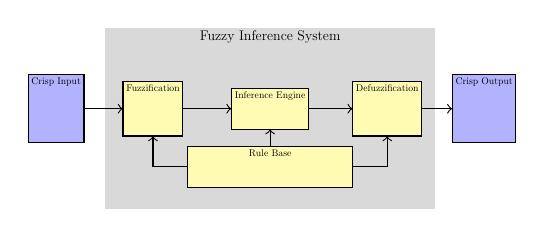
\begin{tikzpicture}[scale=0.35, transform shape]
    \node[fill=gray!30,text depth = 6cm,minimum width=12cm,font=\Large] (main){Fuzzy Inference System};
    \node[draw,fill=yellow!30, text depth=1cm] at ([yshift=1em]main.center)(infer){Inference Engine};
    \node[draw,fill=yellow!30, text depth=1cm, minimum width=6cm] at ([yshift=-5em]main.center)(rb){Rule Base};
    \node[draw,fill=yellow!30, text depth=1.5cm] at ([xshift=5em, yshift=1em]main.west)(fuzz){Fuzzification};
    \node[draw,fill=yellow!30, text depth=1.5cm] at ([xshift=-5em, yshift=1em]main.east)(defuzz){Defuzzification};
    \node[draw,fill=blue!30, text depth=2cm] at ([xshift=-5em, yshift=1em]main.west)(inp){Crisp Input};
    \node[draw,fill=blue!30, text depth=2cm] at ([xshift=5em, yshift=1em]main.east)(outp){Crisp Output};

    \node at ([xshift=5em, yshift=-5em]main.west)(ghostleft){};
    \node at ([xshift=-5em, yshift=-5em]main.east)(ghostright){};

    \draw[->](inp.east) -- (fuzz.west);
    \draw[->](fuzz.east) -- (infer.west);
    \draw[->](infer.east) -- (defuzz.west);
    \draw[->](defuzz.east) -- (outp.west);
    \draw[->](rb.north) -- (infer.south);
    \draw[->](rb.west) -- (ghostleft.center) -- (fuzz.south);
    \draw[->](rb.east) -- (ghostright.center) -- (defuzz.south);
\end{tikzpicture}
